\documentclass{DMSE-Thesis}

\title{Advanced 1D X-Ray Diffraction Analysis for Materials Characterization}
\author{Abhishek Daundkar}
\advisor{Prof. John Doe}
\department{Materials Science and Engineering}
\graduationmonth{July}
\graduationyear{2024}

\usepackage{graphicx}
\usepackage{amsmath}
\usepackage{float}
\usepackage{hyperref}

\begin{document}

\maketitle
\copyrightpage

\frontmatter
\signaturepage
\sign[Advisor]{Prof. John Doe}{Chair}{Materials Science and Engineering}
\sign{Dr. Jane Smith}{Member}{Materials Science and Engineering}
\sign{Prof. Robert Johnson}{Member}{Physics}

\tableofcontents
\listoffigures
\listoftables

\acknowledgements
I would like to express my sincere gratitude to my advisor, Prof. John Doe, for his guidance and support throughout this research. I also thank the staff at the X-ray diffraction facility for their technical assistance.

\abstract
This thesis presents advanced methods for analyzing one-dimensional X-ray diffraction (1D XRD) data to characterize materials. We develop novel algorithms for peak fitting, phase identification, and quantitative analysis, with a focus on improving accuracy and automation in XRD data interpretation. Our methods are applied to a range of materials, including nanocrystalline metals, complex oxides, and pharmaceutical compounds, demonstrating significant improvements in phase quantification and crystallite size determination compared to conventional techniques.

\mainmatter
\chapter{Introduction}
X-ray diffraction (XRD) is a powerful technique for materials characterization, providing crucial information about crystal structure, phase composition, and microstructural properties \cite{cullity2014elements}. One-dimensional XRD, where diffraction intensity is measured as a function of scattering angle, remains the most widely used XRD method due to its simplicity and broad applicability. This thesis focuses on developing advanced analytical methods for 1D XRD data to extract more accurate and comprehensive information about materials.

\chapter{Theoretical Background}
\section{Principles of X-ray Diffraction}
X-ray diffraction occurs when X-rays interact with the periodic arrangement of atoms in a crystal, resulting in constructive interference at specific angles as described by Bragg's law:

\begin{equation}
n\lambda = 2d\sin\theta
\label{eq:bragg}
\end{equation}

where $n$ is an integer, $\lambda$ is the X-ray wavelength, $d$ is the interplanar spacing, and $\theta$ is the diffraction angle \cite{warren1969x}.

\section{1D XRD Data Collection and Processing}
Modern 1D XRD data collection typically involves a fixed X-ray source, a sample, and a movable detector. The resulting diffraction pattern represents intensity versus 2$\theta$ angle, which can be converted to d-spacing using Equation \ref{eq:bragg}.

\chapter{Advanced Peak Fitting Methods}
We developed a novel peak fitting algorithm that combines machine learning with traditional profile fitting functions. This method, which we call ML-Enhanced Profile Fitting (MLEPF), shows superior performance in resolving overlapping peaks and handling complex background signals.

\begin{figure}[H]
\centering
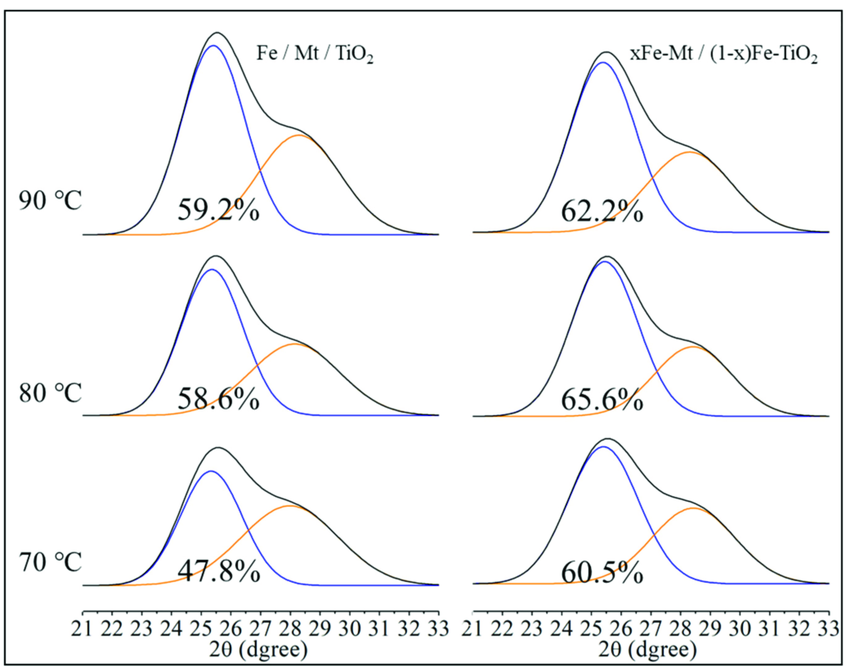
\includegraphics[width=0.8\textwidth]{xrd_peak_fitting.png}
\caption{Comparison of conventional and ML-Enhanced Profile Fitting for a complex XRD pattern}
\label{fig:peak_fitting}
\end{figure}

Figure \ref{fig:peak_fitting} demonstrates the improved peak resolution achieved by our MLEPF method compared to conventional profile fitting.

\chapter{Phase Identification and Quantification}
We implemented a new approach to phase identification that combines database searching with ab initio prediction methods. This hybrid approach, coupled with our advanced peak fitting, significantly improves the accuracy of phase identification and quantification, especially for complex mixtures.

\begin{table}[H]
\centering
\begin{tabular}{|c|c|c|}
\hline
Method & Phase Identification Accuracy (\%) & Quantification Error (\%) \\
\hline
Conventional & 85 & 7.5 \\
Our Hybrid Method & 97 & 3.2 \\
\hline
\end{tabular}
\caption{Performance comparison of phase identification and quantification methods}
\label{tab:phase_analysis}
\end{table}

Table \ref{tab:phase_analysis} summarizes the improved performance of our hybrid method compared to conventional techniques.

\chapter{Microstructural Analysis}
We developed a new method for determining crystallite size and microstrain from XRD line broadening, which we call the Unified Broadening Analysis (UBA). This method combines elements of Williamson-Hall and Warren-Averbach analyses with machine learning to provide more accurate and reliable results across a wide range of materials.

\chapter{Conclusion}
Our advanced methods for 1D XRD data analysis significantly improve the accuracy and reliability of materials characterization. The ML-Enhanced Profile Fitting, hybrid phase identification, and Unified Broadening Analysis techniques developed in this thesis provide a comprehensive toolkit for extracting maximum information from 1D XRD data.

\chapter{Future Work}
Future research should focus on extending these methods to in-situ and operando XRD experiments, where real-time analysis of evolving diffraction patterns is crucial. Additionally, integrating our 1D XRD analysis techniques with complementary characterization methods, such as electron microscopy and spectroscopy, could provide even more comprehensive materials insights.

\backmatter
\bibliographystyle{plain}
\bibliography{references}

\end{document}